\documentclass[12pt,a4paper]{article}

% Mathematics
\usepackage{amsmath,amssymb}
\usepackage{slashed}

% Graphics
\usepackage{graphicx}
\usepackage{epsfig}
\usepackage{epstopdf}

% Tables and page layout
\usepackage{multirow}
\usepackage{array}
\usepackage{needspace}
\newcolumntype{P}[1]{>{\raggedright\arraybackslash}p{#1}}
\usepackage{placeins}
\setlength{\parskip}{10pt}

% Text formatting and URLs
\usepackage{microtype}
\setlength{\emergencystretch}{3em}
\usepackage{url}

% Colors and cross-document citations
\usepackage[dvipsnames]{xcolor}

% Hyperlinks (load near the end)
\usepackage[
    colorlinks=true,
    citecolor=purple,
    linkcolor=blue
]{hyperref}

\begin{document}

\subsection*{Response to the Referee}

\noindent Dear Editor,

This paper considers an anomaly-free, renormalizable model of an additional Abelian
gauge boson \(A'\) with chiral couplings to muons and taus. In this model, vector-like
leptons and a scalar field \(S\) are introduced to construct the ultraviolet completion
of the axial \(U_A(1)_{L_{\mu-\tau}}\) gauge theory. The phenomenology of the \(A'\) in
the axial limit is studied, and the relevant experimental constraints are discussed.
The paper also discusses a possible future muon-collider probe as a complementary test of the chiral interaction structure.

The referee summarizes our work as follows:

\begin{quote}
\itshape
The authors construct an anomaly-free, renormalizable model in which an additional Abelian gauge field \(A'\) has chiral couplings to muons and taus. This model realizes a limit where the \(A'\) coupling to the \(\mu-\tau\) current is axial. The second goal of the paper is to examine the phenomenology of this model in the axial limit.

The paper presents results that are useful for the model building community. However, I have some significant reservations about key points that either should be included or otherwise justified in being excluded from the manuscript. These are explained below. Revisions for these major points (even if only to clarify why they are not issues) are required before the paper is at the level of a PRD manuscript.
\end{quote}

We sincerely thank the referee for the positive assessment of the model-building construction and for identifying issues that require further clarification or quantitative analysis. We respond to each point below.

\medskip
\noindent {\bf Major Points 1)}. \begin{quote}\itshape
Phenomenology of the \(S\) scalar. The second half of the paper reviews a set of experimental bounds on only an effective theory of the \(A'\) axially coupled to the \(L_{\mu-\tau}\) current. This leaves a major gap between these two parts of the paper: the authors show that their UV theory requires a scalar \(S\) that cannot be arbitrarily decoupled from the low-energy dynamics, e.g. from Eq. (34) which states that \(m_S^2 < 4\pi\left(m_{A'}/(2g_X)\right)^2\).\end{quote}

\noindent {\bf Reply.}
The scalar \(S\) is not omitted from the UV phenomenology. The manuscript constructs the symmetry-breaking sector, derives the radial-scalar mass and its lepton interactions, and examines the scalar-sector consistency and experimental constraints before specializing the second part to the axial-current observables of \(A'\). Figure~2 is therefore an analysis of the \(A'\) effective current on a specified scalar-suppressed benchmark, not a scalar-free replacement of the UV theory.

With the scalar-potential convention
\[
V(S)=-\mu_S^2|S|^2+\lambda_S|S|^4,
\]
the UV construction gives
\[
m_{A'}=2g_Xv_s,\qquad
m_s=\sqrt{2\lambda_S}\,v_s,\qquad
y_{s\ell\ell}\simeq\frac{m_\ell}{v_s}
=\frac{2g_Xm_\ell}{m_{A'}},
\quad \ell=\mu,\tau.
\]
Thus, at fixed \((m_{A'},g_X)\), the scalar--lepton couplings are fixed by the symmetry-breaking scale, whereas the physical scalar mass is controlled by \(\lambda_S\). Equivalently,
\[
\lambda_S=\frac{2g_X^2m_s^2}{m_{A'}^2},
\qquad
m_s\leq\sqrt{2\lambda_S^{\max}}\,v_s
=\sqrt{\frac{\lambda_S^{\max}}{2}}\frac{m_{A'}}{g_X}
\]
when the perturbativity criterion \(\lambda_S\leq\lambda_S^{\max}\) is imposed.

For the reference choice \(\lambda_S^{\max}=4\pi\) and \(m_s\gtrsim10\,\mathrm{GeV}\), the scalar-suppressed benchmark therefore has the point-dependent range
\[
10\,\mathrm{GeV}\lesssim m_s\leq\sqrt{8\pi}\,v_s,
\qquad
v_s\gtrsim1.995\,\mathrm{GeV},
\qquad
m_{A'}\gtrsim(3.99\,\mathrm{GeV})\,g_X.
\]
This is the theoretical consistency condition checked at each point in Fig.~2. The scalar mass is consequently not an unconstrained parameter: its upper value follows from perturbativity once \((m_{A'},g_X)\) and the scalar benchmark are specified. The mass-dependent scalar searches are discussed separately below.

For clarity, we summarize selected, non-exhaustive low-mass constraints in the scalar-coupling parameterization relevant to this model. The direct entries constrain \(y_{s\mu\mu}\), not \(g_X\) directly; fifth-force tests are noted separately because their translation depends on loop-induced couplings to ordinary matter and UV matching. For the ultralight binary-pulsar entry, we use Liu and Tang's explicit scalar-mediator analysis, which defines the interaction \(g_{\phi\mu}\phi\bar\mu\mu\) and reports the 95\% CL periastron-advance limit in Fig.~5~\cite{Liu:2025zuz}. We quote the reported sensitivity interval and best-sensitivity point, rather than treating the best point as a uniform bound throughout that interval. The \(L_\mu-L_\tau\) vector-mediator constraint in Ref.~\cite{Dror:2019uea} is not transferred as a direct scalar-Yukawa bound:
\begin{center}
\small
\begin{tabular}{P{0.28\linewidth}P{0.39\linewidth}P{0.20\linewidth}}
\hline
Scalar-mass range & Published constraint & Approximate bound / applicability for \(y_{s\mu\mu}\)\\
\hline
\(10^{-17}\,\mathrm{eV}\lesssim m_s\lesssim2\times10^{-15}\,\mathrm{eV}\) & Binary-pulsar periastron advance (95\% CL), ultralight scalar~\cite{Liu:2025zuz} & \(\mathcal{O}(10^{-21})\) at the best-sensitivity point \(m_s\simeq4\times10^{-16}\,\mathrm{eV}\)\\
\(m_s\lesssim10^{-2}\,\mathrm{eV}\) & Fifth-force tests via loop-induced ordinary-matter couplings~\cite{Fiorillo:2026wso,Hoskins:1985tn,Kapner:2006si,Blakemore:2021zna} & No universal direct \(y_{s\mu\mu}\) limit quoted\\
\(m_s\lesssim1\,\mathrm{keV}\) & Neutron-star cooling~\cite{Fiorillo:2026wso} & \(\lesssim7.4\times10^{-14}\)\\
\(m_s\lesssim1\,\mathrm{keV}\) & SN~1987A cooling (conservative cold-SN model)~\cite{Fiorillo:2026wso,Caputo:2021rux} & \(\lesssim4.2\times10^{-9}\)\\
\(100\,\mathrm{keV}\lesssim m_s\lesssim\mathcal{O}(10)\,\mathrm{MeV}\) & Diffuse supernova \(\gamma\)-ray background~\cite{Caputo:2021rux} & \(\lesssim4\times10^{-11}\)\\
\hline
\end{tabular}
\end{center}
These are approximate, source-dependent constraints, not a combined exclusion band. The neutron-star cooling and SN~1987A cooling entries use the scalar column in Fiorillo et al.'s Table~1 for the stated low-mass regime~\cite{Fiorillo:2026wso}; the diffuse-supernova-\(\gamma\)-ray plateau is taken from Caputo et al. and applies for masses above approximately \(100\,\mathrm{keV}\) in their reference setup~\cite{Caputo:2021rux}. The fifth-force row flags the loop-induced scalar-to-proton recast shown in Fiorillo et al.'s Fig.~1~\cite{Fiorillo:2026wso}; we do not compress that mass-dependent result into a single direct \(y_{s\mu\mu}\) limit, since translating it to the present UV benchmark requires matching the induced ordinary-matter coupling. None of these entries is a direct, model-independent bound on \(g_X\).
\[
g_X<\frac{y_{\max}m_{A'}}{2m_\mu}.
\]
This is the same conditional conversion used in Eq.~(31) of the original manuscript. It is not a model-independent bound on \(g_X\); it applies only when the scalar--muon Yukawa normalization and benchmark assumptions stated above are satisfied.

The table is a source-anchored summary of selected low-mass constraints on the scalar--muon coupling, not a combined scalar--\(A'\) exclusion map. Collider searches are discussed separately below because their interpretation depends on the portal mixing, production rate, branching fractions, widths, and lifetime, including \(s\to A'A'\) when kinematically open.

\begin{figure}[htbp]
\centering
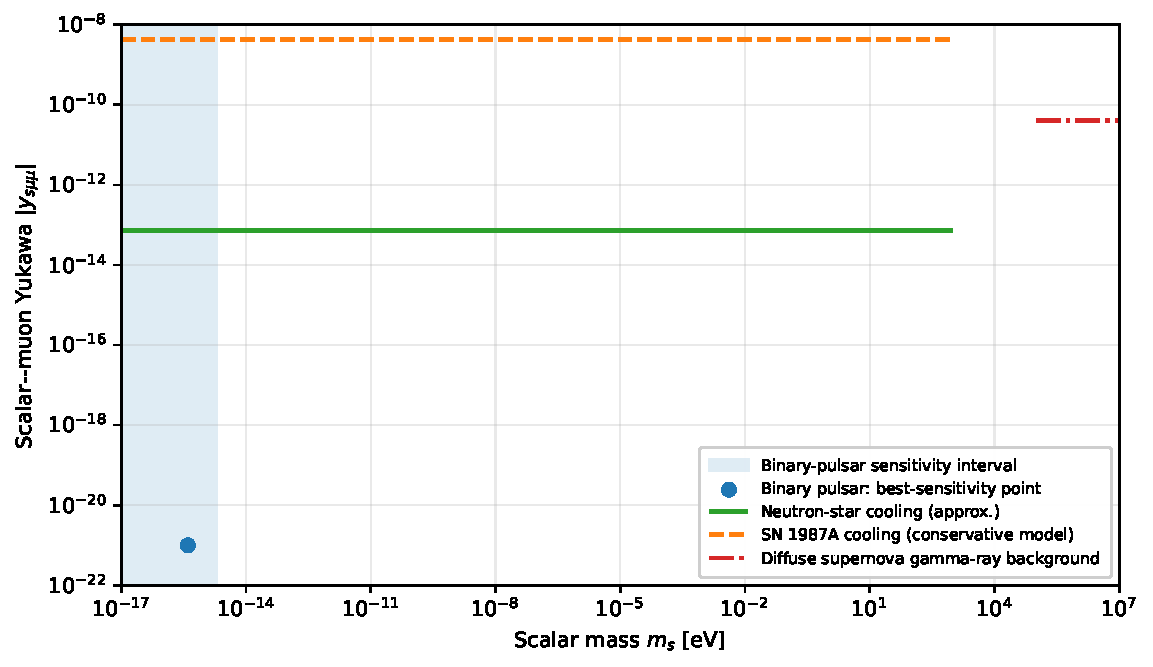
\includegraphics[width=0.96\linewidth]{审稿意见-gpt/当前执行/论文修改与一致性核查/2026-10-28/scalar_coupling_constraints_2026-10-28.pdf}
\caption{Source-anchored summary of selected constraints on the scalar--muon Yukawa coupling \(y_{s\mu\mu}\). The horizontal segments show only source-reported approximate limits in the indicated mass regimes; the binary-pulsar marker gives the published 95\% CL best-sensitivity point and the shaded interval indicates the mass range where that analysis reports its strongest sensitivity. The best-sensitivity value is not treated as a uniform limit across the shaded interval, and the figure is not a digitized combined exclusion contour. In particular, the SN~1987A line shows the free-streaming cooling threshold only and does not represent the full trapping/explosion-energy exclusion. These scalar constraints are not direct limits on the pure-axial \(A'\) current; the UV translation is conditional on \(y_{s\mu\mu}=2g_Xm_\mu/m_{A'}\) and a fixed scalar-mass benchmark within each source's applicability range; the light-scalar bounds shown here do not apply to the \(m_s\gtrsim10\,\mathrm{GeV}\) reference benchmark used for Fig.~2~\cite{Liu:2025zuz,Fiorillo:2026wso,Caputo:2021rux}.}
\label{fig:scalar-muon-constraints-response}
\end{figure}

The intermediate-mass scalar phenomenology is also treated explicitly. BaBar and Belle searched for
\[
e^+e^-\to\tau^+\tau^-s,\qquad
s\to e^+e^-,\,\mu^+\mu^-,
\]
over approximately \(0.04\,\mathrm{GeV}\lesssim m_s\lesssim6.5\text{--}7\,\mathrm{GeV}\). In the mass-proportional benchmark used in these analyses,
\[
\mathcal L\supset-\xi\sum_\ell\frac{m_\ell}{v_h}s\bar\ell\ell,
\qquad \xi=\frac{v_h}{v_s}.
\]
The Belle result \(\xi^{\rm lim}=0.483\) at \(m_s=1\,\mathrm{GeV}\) therefore gives
\[
v_s>\frac{v_h}{\xi^{\rm lim}}\simeq509\,\mathrm{GeV},
\qquad
y_{s\mu\mu}<2.1\times10^{-4},
\]
and, using \(m_{A'}=2g_Xv_s\),
\[
g_X<9.8\times10^{-4}
\left(\frac{m_{A'}}{\mathrm{GeV}}\right)
\]
at \(90\%\) confidence level. This is a direct scalar-search result translated into the UV parameters through the coupling relation derived in the model. The scalar decay widths are also given explicitly: in particular, \(s\to A'A'\) opens for \(m_s>2m_{A'}\) and can change the visible branching fractions relevant to these searches. The B-factory result is thus used with its stated mass-proportional benchmark and the model's scalar decay structure.

The scalar contribution to the muon anomalous magnetic moment is included together with the axial-vector contribution,
\[
\Delta a_\mu=\Delta a_\mu^{A'}+\Delta a_\mu^s,
\qquad
\Delta a_\mu^s=
\frac{y_{s\mu\mu}^2}{8\pi^2}
\int_0^1 dx\,
\frac{x^2(2-x)m_\mu^2}
{m_s^2(1-x)+x^2m_\mu^2}.
\]
For the reference regime \(m_s\gtrsim10\,\mathrm{GeV}\), the scalar term is below \(0.2\%\) of the pure-axial \(A'\) contribution. For lighter \(s\), the positive scalar term can instead compete with, or partially cancel, the negative axial contribution. Accordingly, the \((g-2)_\mu\) contour in Fig.~2 is evaluated for the stated scalar-suppressed benchmark, rather than being applied to arbitrary scalar masses.

These results show how the scalar sector is connected to the second part of the paper: its mass and couplings follow from the UV construction; its mass range is restricted by the scalar self-coupling; low-mass and B-factory searches constrain the corresponding scalar couplings; and its contribution to \((g-2)_\mu\) is included when assessing the effective-current benchmark. The second part therefore presents the \(A'\) axial-current constraints on a specified, perturbatively consistent scalar benchmark; it does not remove \(S\) from the UV theory or treat its phenomenology as absent. The portal benchmark and the associated \(h\)--\(s\) mixing check are addressed separately under Major Point~1.3.


\medskip
\Needspace{8\baselineskip}
\noindent {\bf Major Points 1.1)}. \begin{quote}\itshape
It is thus an odd choice to exclude the scalar from the phenomenology of the effective theory: if the \(S\) is unavoidable at phenomenologically relevant scales, shouldn't one of the main points of the paper be that the only known UV completion of an axial \(L_{\mu-\tau}\) gauge boson has a prediction for a scalar particle in a mass range that can be probed by colliders?\end{quote}

\noindent {\bf Reply.}
The scalar is a physical and potentially testable prediction of the UV completion, and its phenomenology is already included in the manuscript's discussion of the scalar mass, lepton couplings, perturbativity, and direct searches. In particular, BaBar and Belle searched for \(e^+e^-\to\tau^+\tau^-s\), followed by \(s\to e^+e^-\) or \(\mu^+\mu^-\), over approximately \(0.04\,\mathrm{GeV}\lesssim m_s\lesssim6.5\text{--}7\,\mathrm{GeV}\). The mass-proportional benchmark and its translation to \(v_s\), \(y_{s\mu\mu}\), and \((m_{A'},g_X)\) are given in the overall response above.

The Belle~II four-lepton resonance searches extend the relevant resonance-search coverage to approximately \(9\text{--}10\,\mathrm{GeV}\), but the published interpretations cited in the manuscript assume a spin-one mediator. We therefore distinguish these searches from the direct BaBar/Belle scalar limits: the Belle~II mass coverage is relevant context, but it is not applied as a direct exclusion of the radial scalar \(s\). A scalar interpretation would require the scalar-specific production distribution and detector acceptance. For context, generic singlet--Higgs mixing and additional-scalar searches have been studied in Refs.~\cite{Robens:2015singlet,Robens:2020twoSinglets,Boiarska:2019scalarPortal}. These studies provide complementary information on the scalar sector; the connection to the present UV construction is determined by the model-specific mass, coupling, and decay relations summarized above.

The division of emphasis in the paper is consequently physical: the scalar sector is treated through its UV mass and coupling relations and the scalar-specific constraints, while Fig.~2 is reserved for the axial-current phenomenology of \(A'\) in the stated scalar-suppressed benchmark. This keeps the two analyses distinct without omitting the scalar prediction.

\medskip
\noindent {\bf Major Points 1.2)}. \begin{quote}\itshape
What is the range of phenomenologically allowed \(S\) mass including perturbativity limits on \(\lambda\) and a motivated range of \(m_{A'}\) and \(g_X\). For example: perhaps the authors imagine a range of \(m_{A'}\) below some benchmark mass where certain experimental constraints on \(g_X\) become very strong. Then with that set of constraints (which should be stated clearly, see minor point \#1 below), one may give a range of \(m_S\) and comment on the experimental constraints.\end{quote}

\noindent {\bf Reply.}
The manuscript specifies the scalar-mass range point by point through the UV relations, rather than assigning a single scalar mass interval independently of \((m_{A'},g_X)\). In the one-VEV construction,
\[
v_s=\frac{m_{A'}}{2g_X},
\qquad
\lambda_S=\frac{m_s^2}{2v_s^2}
=\frac{2g_X^2m_s^2}{m_{A'}^2}.
\]
For the scalar-suppressed reference benchmark \(m_s\gtrsim10\,\mathrm{GeV}\) and the perturbativity criterion \(\lambda_S\leq4\pi\), the corresponding point-dependent range is
\[
10\,\mathrm{GeV}\lesssim m_s\leq\sqrt{8\pi}\,v_s
=\sqrt{2\pi}\,\frac{m_{A'}}{g_X}.
\]
It requires
\[
v_s\gtrsim\frac{10\,\mathrm{GeV}}{\sqrt{8\pi}}
\simeq1.995\,\mathrm{GeV},
\qquad
m_{A'}\gtrsim(3.99\,\mathrm{GeV})\,g_X.
\]
This is the theoretical consistency boundary represented by the \(v_s\simeq2\,\mathrm{GeV}\) line in Fig.~2. At each plotted point, \(v_s\) is derived and the scalar self-coupling is checked against the perturbativity criterion.

The lower-mass scalar regimes are treated separately through the source-based constraints summarized under Major Point~1 and the direct BaBar/Belle searches discussed under Major Point~1.1. Thus, the manuscript distinguishes the point-dependent perturbative mass range used for the \(A'\) benchmark from the mass-dependent scalar searches. The dashed line is a theoretical consistency condition for the specified \(m_s\gtrsim10\,\mathrm{GeV}\) benchmark, not an experimental exclusion or a universal boundary for every possible scalar-sector choice.

\medskip
\noindent {\bf Major Points 1.3)}. \begin{quote}\itshape
Above (34): the authors ``assume negligible Higgs-portal mixing.'' Is this interaction not generated at loop level? It seems that \(S\)-\(h\) mixing cannot be avoided due to \(\mu\) and \(\tau\) loops. In turn, this seems like it would lead to strong experimental bounds on the UV completion. In fact, once there is mixing, is there not a resonance where the mixing becomes large as \(m_S\to m_h\)? It would be useful to quantify the size of this mixing over the allowed range of \(m_S\). Existing Higgs measurements may set the strongest bounds on the UV completion. If these bounds are obviously negligible (though again, I expect this to be strongly constrained as \(m_S\to m_h\)), then the authors should present this as the justification for ignoring \(m_S\) in the low-energy theory. (Though I am still skeptical that the \(S\) can be ignored since it cannot formally decouple.)\end{quote}

\noindent {\bf Reply.}
We agree that a vanishing Higgs-portal coupling is not enforced by the gauge symmetry: the operator \((H^\dagger H)(S^\dagger S)\) is allowed, so the portal boundary condition must be stated at a matching scale and in a specified renormalization convention. The negligible-portal assumption is therefore used only as a conditional phenomenological benchmark, not as a symmetry-protected statement or a claim that the portal vanishes at every scale.

The general phenomenology of Higgs--singlet mixing, including its impact on the \(125\) GeV Higgs signal strengths and searches for additional scalar states, has already been studied in detail; representative analyses are cited above. This is one reason we do not reproduce a full generic singlet-Higgs analysis in a paper whose main objective is the axial-vector \(A'\) phenomenology. These studies do not, however, determine the physical mixing in our particular UV model, and we do not use them as a substitute for the model-specific loop check.

The zero-momentum effective-potential analysis for the vector-like-lepton (VLL) sector gives, under its stated potential convention,
\[
\lambda_{HS}^{\mathrm{EFT}}(\mu_R)
=\lambda_{HS}^{\mathrm{UV}}(\mu_R)
-\sum_{\ell=\mu,\tau}
\frac{|y_\ell|^2|\lambda_\ell|^2}{8\pi^2}
+\cdots,
\]
where \(y_\ell\) and \(\lambda_\ell\) are the Yukawa couplings in the VLL interaction. This is a conditional zero-momentum threshold relation; it does not determine the finite-momentum off-diagonal self-energy or a physical scalar mixing angle.

To make the portal assumption explicit, we have evaluated the leading VLL threshold at the matching scale \(\mu_M=M_E\),
\[
\Delta\lambda_{HS}^{E}
=-\frac{1}{8\pi^2}\sum_{\ell=\mu,\tau}|y_\ell|^2|\lambda_\ell|^2,
\qquad
\lambda_{HS}^{\mathrm{EFT}}(\mu_M)
=\lambda_{HS}^{\mathrm{UV}}(\mu_M)+\Delta\lambda_{HS}^{E}.
\]
We use \(\lambda_{HS}^{\mathrm{EFT}}(M_E)=0\) as an explicit small-portal reference condition, which requires a nonzero UV portal \(\lambda_{HS}^{\mathrm{UV}}=-\Delta\lambda_{HS}^{E}\). This condition is a benchmark choice, not a symmetry prediction. For illustration, taking \(M_E=20\,\mathrm{TeV}\), \(\theta_{\mu L}=\theta_{\tau L}=10^{-2}\), and the leading seesaw relations gives \(\Delta\lambda_{HS}^{E}\simeq-0.2108\) at \((m_{A'},g_X,v_s)=(10\,\mathrm{GeV},0.0705,70.9\,\mathrm{GeV})\), and \(\Delta\lambda_{HS}^{E}\simeq-0.01067\) at \((63\,\mathrm{GeV},0.1,315\,\mathrm{GeV})\). For these illustrative points only, we additionally impose \(|\lambda_\ell|\leq\sqrt{4\pi}\); this is a theory-consistency benchmark rather than a new exclusion contour in Fig.~2. The comparison demonstrates that setting the UV portal to zero is not equivalent to setting the matched EFT portal to zero, and that the latter must be stated as an input if the small-portal benchmark is retained.

In the present zero-tree-level-mixing setup, the singlet-like field \(s\) has no tree-level \(sWW\) or \(s\bar t t\) vertex; accordingly, direct one-loop \(W\)- or top-quark diagrams do not contribute to \(\Pi_{hs}\) at this order. The leading one-loop off-diagonal contribution instead comes from the charged-lepton/vector-like-lepton sector. We have evaluated this fermion contribution using the full \(2\times2\) charged-lepton/VLL mass-eigenstate matrices, including light-light, light-heavy, heavy-light, and heavy-heavy internal states, and have separated the light-lepton EFT contribution from the hard momentum-dependent term. We use the explicit reference condition \(\lambda_{HS}^{\mathrm{EFT}}(M_E)=0\) stated above; the result is therefore conditional on that matching choice and is not a prediction independent of the renormalized portal boundary.

For illustration, with \(M_E=20\,\mathrm{TeV}\), \(\theta_{\mu L}=\theta_{\tau L}=10^{-2}\), and the same leading-seesaw benchmark inputs used for the threshold check, the matched off-diagonal self-energy at \(p^2=m_h^2\) is
\[
\Pi_{hs}^{\mathrm{matched}}(m_h^2)
\simeq(-0.4133-0.1132i)\,\mathrm{GeV}^2
\]
for \((m_{A'},g_X,v_s)=(10\,\mathrm{GeV},0.0705,70.9\,\mathrm{GeV})\), and
\[
\Pi_{hs}^{\mathrm{matched}}(m_h^2)
\simeq(-0.09300-0.02547i)\,\mathrm{GeV}^2
\]
for \((m_{A'},g_X,v_s)=(63\,\mathrm{GeV},0.1,315\,\mathrm{GeV})\). 

The finite-momentum result does not imply uniformly negligible mixing. At \(m_s=m_h=125.25\,\mathrm{GeV}\), the width-regulated diagnostic \(|\Pi_{hs}/(a-b)|\), with \(a=m_h^2-i m_h\Gamma_h\) and \(b=m_s^2-i m_s\Gamma_s\), is approximately \(9.1\times10^{-4}\) when \(s\to A'A'\) is open and \(\Gamma_s\simeq3.75\,\mathrm{GeV}\). For the benchmark in which \(s\to A'A'\) is closed and \(\Gamma_s\simeq0.159\,\mathrm{MeV}\), the same diagnostic reaches about \(0.197\) at exact degeneracy; the corresponding \(2|\Pi_{hs}/(a-b)|\) diagnostic is about \(0.394\). 

Across the illustrative \(m_s\in[10,150]\,\mathrm{GeV}\) diagnostic scan, the criterion \(2|\Pi_{hs}/(a-b)|\geq0.1\) is not reached in the open-channel benchmark. In the closed-channel benchmark near \(m_s\simeq m_h\), the fixed-self-energy diagnostic exceeds this criterion only within a narrow band of approximately \(7.5\,\mathrm{MeV}\) on either side of \(m_h=125.25\,\mathrm{GeV}\). The estimate holds the matched \(\Pi_{hs}(m_h^2)\) fixed while varying \(m_s\) and the tree-level singlet width; it is a diagnostic approximation, not a self-consistent two-pole solution or an experimental exclusion interval. This narrow band is not covered by the small-mixing approximation. The scalar \(S\) remains part of the UV construction, and Fig.~2 represents the specified small-portal, pure-axial effective-current benchmark rather than a global UV exclusion.



\medskip
\noindent {\bf Major Points 2)}. \begin{quote}\itshape
Motivating the range of effective theory parameters. To further aid in the comparison between the UV theory and the two-parameter low-energy theory, it would be useful to explicitly state in one place (perhaps in a table or a figure like Fig. 2) the range of the effective model parameters that are feasible. The main phenomenological results are in Fig. 2, but it was not clear why this range of couplings and \(A'\) masses were chosen: are values outside this range not allowed? What, if anything, does the perturbativity of the UV theory impose on the effective parameters?\end{quote}

\noindent {\bf Reply.}
We thank the referee for asking us to motivate the parameter window and to distinguish the low-energy effective-current analysis from the UV theory. The ranges displayed in Fig.~2 are
\[
10^{-3}\,\mathrm{GeV}\leq m_{A'}\leq10^2\,\mathrm{GeV},
\qquad
10^{-6}\leq g_X\leq10^{-1}.
\]
They define the plotting window adopted for this comparison, not universal theoretical or experimental boundaries.

The mass interval is chosen to display several distinct regimes represented by the constraints actually included in Fig.~2, rather than to imply uniform experimental coverage across the entire interval. The PIENU pion-decay search is kinematically sensitive for \(m_{A'}<m_{\pi^+}-m_\mu\simeq33.9\,\mathrm{MeV}\)~\cite{PIENU:2021clt,Altmannshofer:2026opc}, while the NA62 kaon-decay channel reaches \(m_{A'}<m_{K^+}-m_\mu\simeq388\,\mathrm{MeV}\) and is shown as an indicative recast~\cite{NA62:2021bji}. CCFR and CHARM~II neutrino-trident measurements provide complementary low-energy constraints~\cite{CCFR:1991lpl,geiregat1990first}; the NA64\(_\mu\) beam-dump result probes the sub-GeV region~\cite{NA64:2024nwj}; and the BaBar and Belle~II four-muon searches extend the visible-resonance coverage to the several-GeV range, while CMS reaches masses of order tens of GeV~\cite{BaBar:2016sci,Belle-II:2024wtd,CMS:2018yxg}. The \((g-2)_\mu\) comparison supplies a separate low-energy precision constraint~\cite{Muong-2:2025xyk}. Thus, the MeV--\(100\,\mathrm{GeV}\) interval spans the different mass regimes relevant to the analyses included in the paper; it does not mean that every experiment covers every mass in this interval. In particular, \(1\,\mathrm{MeV}\) and \(100\,\mathrm{GeV}\) are the chosen endpoints of the displayed mass window, not experimentally established lower and upper cutoffs.

The coupling endpoints \(10^{-6}\) and \(10^{-1}\) are likewise numerical choices for the scan and display. The upper endpoint \(g_X=0.1\) lies well below the usual gauge-coupling perturbativity criterion \(g_X\lesssim\sqrt{4\pi}\), but perturbativity does not select \(0.1\) as a maximum. The lower endpoint \(10^{-6}\) is not a universal lower bound from theory or experiment. Neither coupling endpoint is a strict physical boundary.

For clarity, the scan variables and their UV interpretation are summarized here:
\begin{center}
\small
\begin{tabular}{@{}P{0.19\linewidth}P{0.34\linewidth}P{0.39\linewidth}@{}}
\hline
Quantity & Range or relation & Interpretation\\
\hline
\(m_{A'}\) & \(10^{-3}\)--\(10^2\,\mathrm{GeV}\) & Chosen plotting window spanning several experimentally probed regimes; not a universal mass bound.\\
\(g_X\) & \(10^{-6}\)--\(10^{-1}\) & Chosen scan endpoints; the upper edge is below the usual perturbativity criterion, but neither endpoint is a universal allowed-range boundary.\\
\(v_s\) & \(v_s=m_{A'}/(2g_X)\) & Derived from each selected \((m_{A'},g_X)\) point, not an independent scan variable.\\
\(\lambda_S\) & \(\lambda_S=m_s^2/(2v_s^2)=2g_X^2m_s^2/m_{A'}^2\) & Scalar self-coupling in the stated small-portal benchmark; its perturbativity condition must be checked separately.\\
\(m_s\) benchmark & \(m_s\geq10\,\mathrm{GeV}\) for the scalar-suppressed reference case & Reference scalar-mass benchmark used to evaluate the UV consistency condition.\\
\hline
\end{tabular}
\end{center}

In the scalar-mass convention used in the manuscript, imposing \(\lambda_S\leq\lambda_S^{\max}\) gives
\[
m_s\leq\sqrt{2\lambda_S^{\max}}\,v_s.
\]
For the illustrative choice \(\lambda_S^{\max}=4\pi\), this becomes \(m_s\leq\sqrt{8\pi}\,v_s\). Consequently, the reference benchmark \(m_s\geq10\,\mathrm{GeV}\) requires
\[
v_s\geq\frac{10\,\mathrm{GeV}}{\sqrt{8\pi}}
\simeq1.995\,\mathrm{GeV},
\qquad
m_{A'}\gtrsim(3.99\,\mathrm{GeV})\,g_X.
\]
This is the same \(v_s\simeq2\,\mathrm{GeV}\) boundary shown by the dashed line in Fig.~2: the side with \(v_s<2\,\mathrm{GeV}\) does not satisfy the chosen \(m_s\geq10\,\mathrm{GeV}\), \(\lambda_S\leq4\pi\) benchmark. This is a conditional theoretical consistency requirement, not an experimental exclusion. A point that fails it does not support this scalar benchmark; it is not thereby excluded from every possible realization of the UV model if the scalar mass or scalar-sector assumptions are changed. Within the displayed range \(g_X\leq0.1\), the gauge-coupling perturbativity criterion is not the limiting condition. The scalar self-coupling condition instead imposes a point-dependent check once \(m_s\) is specified.


The scalar bounds discussed under Major Point~1 constrain \(y_{s\mu\mu}\) directly. They can be translated into the \((m_{A'},g_X)\) plane only for a specified scalar-mass benchmark and under the UV relation \(y_{s\mu\mu}=2g_Xm_\mu/m_{A'}\); they are not direct, benchmark-independent limits on the pure-axial \(A'\) current.

For clarity, Fig.~2 should be read according to the following distinctions:
\begin{center}
\small
\begin{tabular}{p{0.30\linewidth}p{0.62\linewidth}}
\hline
Region or condition & Interpretation \\
\hline
Excluded by a contour shown in Fig.~2 & Excluded under the assumptions of that particular effective-current constraint. \\
Not excluded by the contours shown & Survives the constraints displayed in Fig.~2; this alone does not establish every UV consistency condition. \\
Fails the chosen scalar benchmark & Does not satisfy \(m_s\geq10\,\mathrm{GeV}\) together with \(\lambda_S\leq4\pi\) at that point; other scalar-sector choices are not ruled out by this condition alone. \\
Outside the plotted window & Not forbidden by the scan endpoints themselves; no exclusion or viability claim follows solely from being outside the displayed axes. \\
\hline
\end{tabular}
\end{center}
The contours therefore communicate the constraints actually applied, while the axis endpoints specify the range chosen to present the phenomenology.


\medskip
\noindent {\bf Major Points 3)}.

\begin{quote}\itshape
Are neutrino oscillations possible? The Standard Model is defined with only left-handed neutrinos because of the possibility that neutrinos are their own antiparticle. In such a case neutrino masses are generated through, e.g. through the Weinberg operator.
\end{quote}

\medskip
\noindent {\bf Reply to Point 3.1}

\begin{quote}\itshape
In this model, \(U_A(1)_{L_{\mu-\tau}}\) invariance allows Weinberg operators for each generation. However, it appears that both the Yukawa matrices and neutrino masses must be aligned and therefore a non-trivial PMNS matrix does not appear to be possible.
\end{quote}

\noindent {\bf Reply.}

We have checked the operator-selection rules for the charge assignment of the minimal construction,
\[
Q'(L_e,L_\mu,L_\tau)=(0,+Q_\ell,-Q_\ell),\qquad
Q'(H)=0,\qquad Q'(S)=2Q_\ell.
\]
After \(S\) acquires a vacuum expectation value, the residual \(Z_2\) makes the electron-flavor fields even and the \(\mu\)- and \(\tau\)-flavor fields odd. At the effective-field-theory (EFT) level, the Weinberg operators \((L_eH)(L_eH)\) and \((L_\mu H)(L_\tau H)\) are allowed at dimension five. The diagonal operators \((L_\mu H)(L_\mu H)\) and \((L_\tau H)(L_\tau H)\) require one \(S^\dagger\) or \(S\) insertion, respectively, and therefore first occur at dimension six. The \(e\mu\) and \(e\tau\) entries remain forbidden for any number of \(S\) and \(S^\dagger\) insertions, because these insertions change the charge only by even multiples of \(Q_\ell\).

If these symmetry-allowed EFT operators are included, the resulting neutrino mass matrix has the block form
\[
M_\nu=
\begin{pmatrix}
A&0&0\\
0&B\varepsilon&C\\
0&C&D\varepsilon
\end{pmatrix},
\qquad \varepsilon\sim v_s/\Lambda,
\]
while the charged-lepton Yukawa matrix has the corresponding structure
\[
Y_\ell=
\begin{pmatrix}
c&0&0\\
0&a\varepsilon&b\\
0&b'&d\varepsilon
\end{pmatrix},
\]
where the \(\mu\)--\(\tau\) entries \(b,b'\) are allowed without an \(S/\Lambda\) suppression. Both matrices preserve the \(\{e\}\oplus\{\mu,\tau\}\) block decomposition. Consequently, up to a permutation of the neutrino mass eigenstates and phase conventions,
\[
U_{\rm PMNS}=U_L^\dagger U_\nu
=\operatorname{diag}\!\left(1,U_{23}\right).
\]
The PMNS matrix is therefore not necessarily the identity: a nontrivial rotation within the \(\mu\)--\(\tau\) sector may remain. However, one mass eigenstate is purely electron flavor and the other two have no electron-flavor component. Thus the nonzero electron-flavor admixtures required by oscillation data (in particular, the observed nonzero \(\theta_{12}\) and \(\theta_{13}\)) cannot be reproduced by the minimal charge assignment.

This is a limitation of the minimal construction, not a solved neutrino-mass mechanism. The Weinberg operators above are symmetry-allowed EFT terms; their allowance does not by itself show that the minimal renormalizable UV Lagrangian generates them or fixes their coefficients. We therefore do not claim that the minimal field content explains the observed neutrino oscillations or reproduces the full PMNS matrix.

\medskip
\noindent {\bf Reply to Point 3.2}

\begin{quote}\itshape
Perhaps a full model would require right-handed neutrinos. These would now be charged under \(U_A(1)_{L_{\mu-\tau}}\), which likely means the second and third generation must appear as vectorlike combinations. However, it seems to me that mixing between generations is prohibited by \(U_A(1)_{L_{\mu-\tau}}\).
\end{quote}

\noindent {\bf Reply.}

Introducing right-handed neutrinos alone does not remove the obstruction. Since \(S\) is even under the residual \(Z_2\), the allowed Dirac and Majorana mass matrices remain block diagonal between the electron-flavor sector and the \(\mu\)--\(\tau\) sector. The type-I seesaw relation \(M_\nu=-m_D M_R^{-1}m_D^T\) preserves this block structure and therefore does not generate the missing electron-flavor mixing.

Related gauged \(L_\mu-L_\tau\) constructions that address neutrino masses and mixing are discussed by Heeck and Rodejohann, Phys. Rev. D \textbf{84}, 075007 (2011)~\cite{Heeck:2011wj}, and Asai, Hamaguchi and Nagata, Eur. Phys. J. C \textbf{77}, 763 (2017)~\cite{Asai:2017ryy}. These are examples of model-dependent neutrino-sector constructions; because their field content and charge assignments are not identical to those of the present axial model, their results cannot be transferred to the minimal construction without extending its neutrino sector.

An additional scalar with an odd \(U_A(1)\) charge and a nonzero vacuum expectation value could break the residual selection rule and allow electron--muon and electron--tau mixing. This would change the field content rather than solve the problem within the minimal construction. We therefore retain the existing model and restrict its claim to the anomaly-free gauge and charged-lepton construction and its axial-vector phenomenology.

\medskip
\noindent {\bf Overall response to Major Point 3.}

\begin{quote}\itshape
Thus it is not obvious to me how neutrino oscillations can be included in this framework. If there is a simple solution, the authors should include it. If there is a known less-simple solution in the literature, the authors should cite this. Otherwise, at best this will be a confusing point. At worst, it would make the construction inconsistent with neutrino oscillation experiments.
\end{quote}

\noindent {\bf Reply.}

We agree that the minimal construction, with the stated field content and charge assignments, does not reproduce the observed PMNS matrix and should not be presented as a complete model of neutrino oscillations. More precisely, the allowed mass matrices are block diagonal rather than necessarily proportional to the identity: \(\mu\)--\(\tau\) mixing may occur, but the electron-flavor admixtures required by oscillation data are absent. Right-handed neutrinos alone do not remove this obstruction; related constructions in the literature illustrate possible extensions but do not establish a solution within the field content adopted here. We therefore do not add new particles for this revision or claim that the minimal construction is compatible with the full neutrino-oscillation data. The paper's scope remains the anomaly-free gauge and charged-lepton construction and its specified axial-vector effective-current phenomenology. This defines the scope of the present construction: the anomaly-free gauge and charged-lepton sector and its axial-vector phenomenology, rather than a complete neutrino-mass and oscillation model.

\medskip
\noindent {\bf 4)}.
\begin{quote}\itshape
Is this the full set of experimental constraints? The second half of the manuscript presents a set of experimental bounds on the two-parameter effective \(A'\) model. It is not obvious if this is the full set of constraints on the model. (See also point \#1 above: I would have liked to see a section discussing the bounds on the \(S\) within this model since it cannot be decoupled.) The following experimental bounds seem like they could be relevant. It would be helpful to either include them or justify why they are subdominant to the experiments presented.
\end{quote}

\noindent {\bf Reply.}

The contours in Fig.~2 constrain the specified two-parameter pure-axial effective-current benchmark; they are not presented as an exhaustive global classification of every point in the UV model. We address the additional issues raised here by summarizing the scalar constraints under Major Point~1, estimating the momentum-dependent kinetic mixing, quantifying the leading effects of the finite vector component, and distinguishing the supernova contributions governed by the unchanged neutrino current from those sensitive to the charged-muon current. The conclusions below are stated for the explicit benchmark and mass regimes in which the corresponding comparison applies.

\medskip
\noindent {\bf 4.1)}.
\begin{quote}\itshape
Neutrino oscillation observations. See point \#3 above. It appears that this model predicts a unit PMNS matrix, which is inconsistent with neutrino oscillations.
\end{quote}

\noindent {\bf Reply.}

As explained in our response to Major Point~3, the minimal construction yields a block-diagonal PMNS matrix, up to mass-eigenstate ordering: a nontrivial \(\mu\)--\(\tau\) rotation may occur, but the electron-flavor admixtures required by the observed nonzero \(\theta_{12}\) and \(\theta_{13}\) are absent. This is the same selection-rule result and scope statement established in our response to Major Point~3.

\medskip
\noindent {\bf 4.2)}.
\begin{quote}\itshape
There is no quantitative estimate of the amount of kinetic mixing generated with the ``benchmark'' choices of \(\theta\leq10^{-2}\). The authors make the insightful point that kinetic mixing goes to zero in the axial limit, but because this limit is tied to the size of the mixing (the mass of the vectorlike leptons), for the above benchmark there is non-zero kinetic mixing. It would be useful to have parametric estimates of the amount of kinetic mixing one expects so that readers may compare to experimental bounds. One could invoke parametric expressions in the literature for the relevant loop diagrams.
\end{quote}

\noindent {\bf Reply.}

We agree that a vanishing kinetic-mixing coefficient at the heavy-vector-like-lepton matching scale does not, by itself, quantify the residual photon--\(A'\) polarization relevant to experiments. The degenerate heavy-VLL threshold and the low-energy charged-lepton loop are distinct contributions. For \(M_{E_\mu}=M_{E_\tau}\), the one-loop heavy threshold proportional to \(\ln(M_{E_\mu}^2/M_{E_\tau}^2)\) vanishes under the stated charge assignment and matching condition. We take no additional bare low-energy kinetic-mixing term in the benchmark considered here.

For the light-lepton loop, we use the momentum-transfer-dependent kinetic-mixing function studied by Hapitas, Tuckler, and Zhang~\cite{Hapitas:2021kineticMixing}; the timelike threshold behavior is compared with Wang and Zhang~\cite{Wang:2026supernova}. In the equal-mixing benchmark and matching condition used here, the irreducible contribution is
\[
\epsilon_{\gamma A'}(q^2)=
-\frac{e\,g_X\sin^2\theta_R}{2\pi^2}
\int_0^1 dx\,x(1-x)
\log\!\left[
\frac{m_\tau^2-x(1-x)q^2-i0}
     {m_\mu^2-x(1-x)q^2-i0}
\right],
\]
where we have imposed the illustrative equal-mixing benchmark
\(\theta_{\mu R}=\theta_{\tau R}\equiv\theta_R\), for which
\(g_V^\mu=-g_V^\tau=g_X\sin^2\theta_R\). The ultraviolet-sensitive terms cancel between the two light-lepton loops in this equal-mixing limit. At \(q^2=0\), this reduces to
\[
\epsilon_{\gamma A'}(0)=
-\frac{e\,g_X\sin^2\theta_R}{12\pi^2}
\ln\frac{m_\tau^2}{m_\mu^2}
=-\frac{e\,g_X\sin^2\theta_R}{6\pi^2}
\ln\frac{m_\tau}{m_\mu}.
\]
Using \(e=0.3028\), \(m_\mu=105.658~\mathrm{MeV}\), \(m_\tau=1.77686~\mathrm{GeV}\), and \(\theta_R=10^{-2}\), the zero-momentum magnitude is
\[
|\epsilon_{\gamma A'}(0)|\simeq1.44\times10^{-6}|g_X|.
\]
This is a benchmark estimate, not a universal prediction for unequal mixing angles or an arbitrary ultraviolet matching condition.

For an on-shell \(A'\), the relevant timelike argument is \(q^2=m_{A'}^2\). The loop function becomes complex above the charged-lepton pair thresholds; its magnitude is not constant across the scan. A numerical evaluation of the integral gives the following representative values for \(\theta_R=10^{-2}\):
\begin{center}
\small
\begin{tabular}{c|c|c}
\(m_{A'}\) &
\shortstack{\(\left|\epsilon_{\gamma A'}(m_{A'}^2)\right|\)\\ \(/\left|g_X\right|\)} &
\shortstack{\(\left|\epsilon_{\gamma A'}(m_{A'}^2)\right|\)\\ \(/\left|\epsilon_{\gamma A'}(0)\right|\)}\\
\hline
\(10~\mathrm{MeV}\) & \(1.44\times10^{-6}\) & \(1.00\)\\
\(100~\mathrm{MeV}\) & \(1.49\times10^{-6}\) & \(1.04\)\\
\(200~\mathrm{MeV}\) & \(1.82\times10^{-6}\) & \(1.26\)\\
\(212~\mathrm{MeV}\) & \(2.12\times10^{-6}\) & \(1.47\)\\
\(500~\mathrm{MeV}\) & \(1.40\times10^{-6}\) & \(0.97\)\\
\(1~\mathrm{GeV}\) & \(1.08\times10^{-6}\) & \(0.75\)\\
\(3~\mathrm{GeV}\) & \(8.06\times10^{-7}\) & \(0.56\)\\
\(10~\mathrm{GeV}\) & \(5.47\times10^{-8}\) & \(3.79\times10^{-2}\)\\
\(100~\mathrm{GeV}\) & \(4.84\times10^{-10}\) & \(3.35\times10^{-4}\)
\end{tabular}
\end{center}
The value near \(m_{A'}=2m_\mu\) agrees with the approximately \(1.47\) enhancement of the magnitude over its zero-momentum value reported by Wang and Zhang~\cite{Wang:2026supernova}. For the low-mass benchmark, the induced electron-current coupling is of order \(e|\epsilon|\simeq4.4\times10^{-7}|g_X|\). The momentum-dependent expression should be used for on-shell production and decay; spacelike virtual exchange requires evaluating the same function at the relevant spacelike \(q^2\).

For the plotted range \(g_X\leq0.1\), the zero-momentum value satisfies \(|\epsilon_{\gamma A'}(0)|\leq1.44\times10^{-7}\); the largest tabulated on-shell value, near \(m_{A'}=2m_\mu\), is \(|\epsilon_{\gamma A'}|\leq2.12\times10^{-7}\). Below the dimuon threshold, \(A'\) decays predominantly to neutrinos, so invisible-dark-photon searches provide the relevant laboratory comparison. The NA64 missing-energy analysis constrains the kinetic-mixing parameter up to \(m_{A'}\lesssim0.35\,\mathrm{GeV}\), with a mass-dependent sensitivity at roughly the \(\mathcal O(10^{-4})\) scale in the relevant interval~\cite{NA64:2023lightDM}. This is well above the induced value in our benchmark. Thus the loop-induced electron-production channel does not set the leading laboratory bound for the stated parameter range. This estimate assumes \(\theta_{\mu R}=\theta_{\tau R}\) and the stated matching condition; unequal angles require the corresponding threshold matching.

\medskip
\noindent {\bf 4.3)}.
\begin{quote}\itshape
Another way of reframing the above point: the bounds presented are in the pure axial limit. Since the authors present a UV model that only realizes the axial coupling in a decoupling limit, it would be useful to comment on possible experimental bounds on the small vector-like coupling in a model with non-infinite vectorlike fermion masses. If these bounds are always small compared to the axial bounds, this should be stated and justified. The importance of this point is as follows: often bounds are sensitive to the chiral structure of interactions. Sometimes a vector interaction is more tightly constrained than its axial counterpart. Since the authors focus on the phenomenology in the axial limit, one wants to make sure that any small-but-finite vector interaction isn't significant because the constraints on the coupling are orders-of-magnitude larger than the axial coupling.
\end{quote}

\noindent {\bf Reply.}

For \(|\theta_{\ell R}|\leq10^{-2}\), the mass-basis couplings obey
\[
\left|\frac{g_V^\ell}{g_A^\ell}\right|
=\tan^2\theta_{\ell R}\leq1.01\times10^{-4}.
\]
At the scan endpoint \(g_X=0.1\), this corresponds to \(|g_V^\ell|\leq10^{-5}\). The neutrino couplings remain \(g_{\nu_\mu}=+g_X\) and \(g_{\nu_\tau}=-g_X\).

For neutrino trident production, the ratio of the leading Standard-Model interference terms induced by the vector and axial components is parametrically
\[
\left|\frac{C_V\delta C_V}{C_A\delta C_A}\right|
\sim\frac{C_V}{C_A}\tan^2\theta_{\mu R}
\lesssim2.0\times10^{-4},
\qquad C_V\simeq0.96,\quad C_A=\frac12,
\]
at the same momentum transfer, before the distinct finite-\(m_\mu\) response functions are included. For the muon anomalous magnetic moment,
\[
\left|\frac{\Delta a_\mu^{V}}{\Delta a_\mu^{A}}\right|
=\tan^4\theta_{\mu R}\frac{F_V(r)}{F_A(r)}
\lesssim2.1\times10^{-9},
\]
using \(F_V/F_A\leq0.20\) over the mass range considered. These estimates show that the finite vector component does not materially change the leading trident-interference or \((g-2)_\mu\) results for the stated benchmark.

The dimuon width requires one threshold qualification:
\[
\Gamma_V\propto(g_V^\mu)^2(1+2r_\mu)\sqrt{1-4r_\mu},\qquad
\Gamma_A\propto(g_A^\mu)^2(1-4r_\mu)^{3/2},
\quad r_\mu=\frac{m_\mu^2}{m_{A'}^2}.
\]
Away from threshold, the vector-squared contribution is suppressed by \(\tan^4\theta_{\mu R}\leq10^{-8}\); very close to threshold, the additional axial phase-space suppression can make the vector term relevant to the branching fraction. We therefore retain the pure-axial interpretation of Fig.~2 for the benchmark observables above and do not extrapolate it to threshold-sensitive visible-decay observables without the corresponding width factors.

\noindent {\bf 4.4)}.
\begin{quote}\itshape
Are stellar cooling bounds not relevant? See e.g. 2511.09619 for a recent paper on this. If they are not, then this is certainly worth justifying.
\end{quote}

\noindent {\bf Reply.}

Supernova cooling is relevant to the sub-GeV region. The referee-cited analysis is now published as JHEP 06 (2026) 155~\cite{Blinov:2025aha}; a recent update for the conventional vector \(L_\mu-L_\tau\) boson, using the SFHo-18.8 profile, reports SN1987A sensitivity up to \(m_{A'}\sim300~\mathrm{MeV}\) and low-energy-supernova sensitivity up to about \(600~\mathrm{MeV}\), with coupling sensitivity reaching approximately \(1.4\times10^{-10}\) and \(6.4\times10^{-12}\), respectively~\cite{Wang:2026supernova}. These values provide the relevant reference scales for assessing the axial benchmark.

In our model, the tree-level neutrino couplings are the same as in the conventional \(L_\mu-L_\tau\) model,
\[
g_{\nu_\mu}=+g_X,\qquad g_{\nu_\tau}=-g_X.
\]
Consequently, neutrino-coalescence production and the invisible partial widths \(A'\to\nu_\alpha\bar\nu_\alpha\) are unchanged at fixed \((m_{A'},g_X)\). In the cited supernova profile, neutrino coalescence dominates the production luminosity for \(m_{A'}\gtrsim10~\mathrm{MeV}\). Accordingly, for \(10~\mathrm{MeV}\lesssim m_{A'}<2m_\mu\), the published SN1987A cooling result is a useful reference scale: neutrino-coalescence production is unchanged and dominates the luminosity in the cited profile, while \(A'\) decays predominantly to neutrinos. We use this as a benchmark comparison, not as a fully recast exclusion contour for the axial model.

The distinction arises in processes involving the charged-muon current. The semi-Compton process \(\mu\gamma\to\mu A'\) and its inverse absorption depend on whether that current is vector or axial; the vector-model curve is therefore not directly transferable in the low-mass region where semi-Compton production dominates. Above \(m_{A'}=2m_\mu\), the axial and vector dimuon widths also differ in their threshold dependence, affecting visible-decay and low-energy-supernova energy-deposition constraints. In the equal-mixing benchmark, the low-momentum kinetic mixing satisfies \(|\epsilon_{\gamma A'}|/|g_X|\simeq1.4\times10^{-6}\), compared with approximately \(1/70\) in the conventional vector model; the corresponding mixing-induced amplitude and rate are smaller by about \(10^{-4}\) and \(10^{-8}\), respectively.

Thus stellar constraints are not dismissed: the neutrino-coalescence contribution is applicable where it dominates, while the full vector-current supernova exclusion curve is not treated as a universal exclusion of the axial model. This distinction preserves the relevant astrophysical information without applying a bound outside the interaction structure for which it was derived.

\medskip
\noindent {\bf Minor Point 1)}. \begin{quote}\itshape
Range of parameters. The general construction of the model is clearly written, but it is difficult for the reader to envision the mass and coupling range that the authors are targeting. It would be very helpful if the authors decide on a range of \(m_{A'}\) and \(g_X\) of interest. For example: is there a range of masses where experimental or theoretical limits are less constraining? Is there some set of phenomenology that the authors seek to realize with a ``light'' \(A'\)? If so, they should define ``light.'' (See, e.g. the first word of the introduction, which is not defined with respect to any reference mass scale.)\end{quote}

\noindent {\bf Reply.}
The word "light" is not intended to specify a separate quantitative mass regime. The Abstract describes the broader MeV-to-TeV scale, while Fig.~2 displays the specific comparison window
\[
10^{-3}\,\mathrm{GeV}\leq m_{A'}\leq10^2\,\mathrm{GeV},
\qquad
10^{-6}\leq g_X\leq10^{-1}.
\]
The numerical range and the observables included in the analysis, rather than the adjective "light", define the phenomenological domain considered here. The motivation for this window and the complementary experimental coverage are detailed in our response to Major Point~2.

\medskip
\noindent {\bf Minor Point 2)}.
\begin{quote}\itshape
Defining the pure-axial limit. Equation (12) gives the coupling of the \(A'\) to the mass-basis fields. It is here that the ``pure axial coupling'' limit is defined? i.e. \(\theta_{\mu R}\to0\)? If that is the case, it would help to define this as the pure-axial limit, a phrase which is used below (36) but not otherwise quantified.
\end{quote}

\noindent {\bf Reply.}

We agree that the pure-axial limit should be quantified when the mass-basis couplings are introduced in Eq.~(12). In the convention used there, the strict pure-axial limit is \(\theta_{\mu R}\to0\):
\[
g_V^\mu=g_X\sin^2\theta_{\mu R}\to0,
\qquad
g_A^\mu=-g_X\cos^2\theta_{\mu R}\to-g_X.
\]
For finite \(\theta_{\mu R}\), the vector coupling is nonzero, so the interaction is not strictly purely axial. We therefore reserve the term ``pure-axial limit'' for \(\theta_{\mu R}\to0\); the analogous limit in the \(\tau\) sector follows with the charge reversal specified in the model.

\medskip
\noindent {\bf Minor Point 3)}.
\begin{quote}\itshape
Bounds on the vectorlike leptons. Because the mixing angles scale inversely with the vectorlike lepton masses, it would be helpful to present lower limits on these masses. This, in turn, gives an upper limit on the \(\theta_{(\mu,\tau)R}\) mixing angles which then gives an upper limit on the \(A'\) vectorlike coupling to \(L_{\mu-\tau}\). How do these bounds compare with the \(\theta_{(\mu,\tau)(L,R)}\) bounds in equation (27)?
\end{quote}

\noindent {\bf Reply.}

In the decoupling regime, the light--heavy mixing angles scale inversely with the vector-like-lepton masses at fixed off-diagonal mass parameters. After matching to the observed charged-lepton masses, Eqs.~(21) and (23) give
\[
m_\ell\simeq\theta_{\ell L}\theta_{\ell R}M_{E\ell},
\qquad \ell=\mu,\tau.
\]
Combining these relations with the small-mixing condition adopted in Eq.~(27),
\[
|\theta_{\ell L}|,\;|\theta_{\ell R}|\leq10^{-2},
\]
gives the following conditional mass scales at leading order:
\[
M_{E\mu}\gtrsim\frac{m_\mu}{(10^{-2})^2}\simeq1.06~\mathrm{TeV},
\qquad
M_{E\tau}\gtrsim\frac{m_\tau}{(10^{-2})^2}\simeq17.8~\mathrm{TeV}.
\]
For the degenerate choice \(M_{E\mu}=M_{E\tau}\equiv M_E\) in Eq.~(22), the tau relation therefore gives the stronger conditional requirement \(M_E\gtrsim17.8~\mathrm{TeV}\). This follows from imposing the mixing-angle condition and reproducing the charged-lepton masses simultaneously; it is not an independent direct-search mass limit. The separate condition \(M_E>10~\mathrm{TeV}\) in Eq.~(22) is weaker than this combined requirement.

Equation~(27) and the mass relations play different roles: Eq.~(27) bounds each mixing angle individually in the adopted small-mixing setup, whereas the mass relations fix the products \(\theta_{\ell L}\theta_{\ell R}\). A mass relation by itself would not yield an individual upper bound on \(\theta_{\ell R}\). Using the Eq.~(27) condition in the mass-basis couplings,
\[
\begin{gathered}
g_V^\mu=g_X\sin^2\theta_{\mu R},\qquad
g_A^\mu=-g_X\cos^2\theta_{\mu R},\\
g_V^\mu\lesssim10^{-4}g_X,\\
\left|\frac{g_V^\mu}{g_A^\mu}\right|=\tan^2\theta_{\mu R}\lesssim10^{-4}.
\end{gathered}
\]
Thus, the residual vector component is suppressed by at least four orders of magnitude relative to the axial component under the adopted condition. This is a consequence of the small-mixing assumption, not a separate experimental bound; by itself it does not establish that every observable is insensitive to the vector component. We clarify the terminology of Eq.~(27) in our response to Minor Point~4.

\medskip
\noindent {\bf Minor Point 4)}.
\begin{quote}\itshape
Conservative benchmark. Equation (27) is presented as a ``conservative benchmark.'' What does this mean? A benchmark point would be a choice of these mixing angles. A constraint is an upper bound. Eq. (27) is written as an upper bound, but is described as a benchmark. This is not simply semantic: readers would want to understand if \(10^{-2}\) is an experimental upper limit or simply a convenient choice.
\end{quote}

\noindent {\bf Reply.}
Equation~(27) specifies the small-mixing assumption used in the phenomenological analysis; it is neither a benchmark point nor a universal experimental upper limit on all four mixing angles. Under this assumption, mixing-dependent corrections are suppressed at order \(\theta^2\lesssim10^{-4}\), and the residual vector component of the \(A'\) coupling is correspondingly small. The bounds on vector-like leptons depend on their electroweak representation and on the observables considered, so the value \(10^{-2}\) defines the controlled small-mixing regime rather than a direct experimental limit.

\medskip
\noindent {\bf Minor Point 5)}.
\begin{quote}\itshape
What is the purpose of including muon collider bounds? The second half of the paper focuses on existing experimental bounds on the effective theory. It is a strange change in tone to include hypothetical muon collider bounds for future reach. The authors do not justify why a future muon collider is the way to test this model in the future and the section feels like it is tacked on. Most of the section emphasizes that the muon collider search would be a ``standard'' follow up of existing work (Ref 83) and so this section does not seem particularly novel. The authors simply focus on the forward-backward asymmetry. Why not also include polarization asymmetries? Or would there be asymmetries in the \(ee\) versus \(\tau\tau\) final states? Given the first half of the paper, though, it seems that the real ``smoking gun'' for this UV completion is the physics of the \(S\) particle which should be tested in any Higgs-factory phase of a future lepton collider. I feel that this section either adds too little and should be downplayed as an example of future tests, or otherwise should have its own full fledged exploration (which may be a separate paper).
\end{quote}


\noindent {\bf Reply.}
The muon-collider discussion serves as an illustrative future-test example, not as a comprehensive collider study or a projected exclusion analysis. Since \(A'\) couples directly to muons, the process \(\mu^+\mu^-\to\tau^+\tau^-\) provides a complementary probe of the heavier-mass regime. The forward--backward asymmetry is shown because the angular distribution retains sensitivity to the chiral structure even when the total rate is similar for vector and axial interactions.

In the effective-current limit considered here, \(A'\) has no tree-level coupling to electrons, so an \(ee\) final state is not an equivalent direct comparison with \(\tau^+\tau^-\). A systematic study of polarization observables, loop-induced electron couplings, and other flavor-tagged asymmetries would require a separate collider analysis. The scalar \(S\) is a complementary UV target for a future Higgs factory, but no quantitative Higgs-factory reach is inferred from the present \(A'\) study. The angular-distribution result is therefore an example of a possible future chirality-sensitive test, not a discovery or exclusion projection.

\medskip
\noindent {\bf Minor Point 6)}. \begin{quote}\itshape
Terminology. The following points could be improved for clarity.
\end{quote}

\medskip
\noindent {\bf Minor Point 6.1)}. \begin{quote}\itshape
The word ``light'' on page 2 has no reference scale.
\end{quote}

\noindent {\bf Reply.}
As clarified in our response to Minor Point~1, the adjective "light" is not a quantitative mass classification. The Abstract and Fig.~2 state the relevant numerical mass ranges; no additional universal threshold is implied.

\medskip
\noindent {\bf Minor Point 6.2)}. \begin{quote}\itshape
At the bottom of page 11, when referring to Table II, the authors write ``representative bounds.'' What does representative mean? Does it mean these are the most stringent bounds? Are these ``some'' bounds? Is the list ``complete'' in any sense?
\end{quote}

\noindent {\bf Reply.}
By "representative bounds" we mean a selected, non-exhaustive set of published constraints that illustrates the different physical mechanisms relevant to the scalar. It does not mean a complete inventory or the strongest limit at every scalar mass. Direct limits on \(y_{s\mu\mu}\) are distinguished from fifth-force limits that require matching loop-induced couplings to ordinary matter~\cite{Liu:2025zuz,Fiorillo:2026wso,Caputo:2021rux,Hoskins:1985tn,Kapner:2006si,Blakemore:2021zna}. Each entry is interpreted with the production, trapping, and matching assumptions of its source analysis.

\medskip
\noindent {\bf Minor Point 6.3)}. \begin{quote}\itshape
Between page 12--13: ``...do not provide a universal \(g_X\) bound, but they show that the intermediate scalar-mass region cannot simply be assumed unconstrained.'' What does intermediate mass mean? It is also not clear what the intended content of this statement is: are the authors presenting a bound? Why would the reader assume that a new particle in this range would be unconstrained?
\end{quote}

\noindent {\bf Reply.}
The intermediate-mass range refers to the direct BaBar and Belle searches for \(e^+e^-\to\tau^+\tau^-s\), followed by \(s\to e^+e^-\) or \(\mu^+\mu^-\), covering approximately \(0.04\,\mathrm{GeV}\lesssim m_s\lesssim6.5\text{--}7\,\mathrm{GeV}\). These are direct scalar searches, not an assumption that the intermediate-mass region is unconstrained. The Belle benchmark at \(m_s=1\,\mathrm{GeV}\), including its translation to \(v_s\), \(y_{s\mu\mu}\), and \((m_{A'},g_X)\), is given explicitly in our response to Major Point~1. The Belle~II four-lepton searches extend to approximately \(9\text{--}10\,\mathrm{GeV}\), but their published interpretations assume a spin-one mediator and are not applied as direct limits on the radial scalar. For the scalar, the visible branching fractions must also account for \(s\to A'A'\) when \(m_s>2m_{A'}\).

\medskip
\noindent {\bf Minor Point 6.4)}. \begin{quote}\itshape
Below (34): ``we impose Eq. (34) point by point'', it's not clear what is meant by ``point.''
\end{quote}

\noindent {\bf Reply.}
A ``point'' denotes one grid point \((m_{A'},g_X)\) in the parameter scan shown in Fig.~2. At each point, the symmetry-breaking scale is derived from
\[
v_s=\frac{m_{A'}}{2g_X},
\]
rather than varied independently. For a specified scalar mass \(m_s\), the scalar self-coupling is then determined by
\[
\lambda_S
=\frac{m_s^2}{2v_s^2}
=\frac{2g_X^2m_s^2}{m_{A'}^2}.
\]
The condition
\[
\lambda_S\leq\lambda_S^{\max}
\]
is consequently checked at each scan point for the adopted scalar benchmark.

Equation~(34) is checked point by point to test the theoretical consistency of the chosen scalar benchmark; it is not itself an experimental exclusion. The experimental constraints are a separate step.

\medskip
\noindent {\bf Minor Point 6.5)}. \begin{quote}\itshape
Page 21, first paragraph of Section E. What is the ``parameter region of interest''? This wasn't clearly defined anywhere.
\end{quote}

\noindent {\bf Reply.}
We agree that the phrase ``parameter region of interest'' did not specify the mass coverage of the searches considered in Section~III.E. The relevant four-muon searches cover approximately
\[
\begin{aligned}
\text{BaBar}:&\quad 0.212\text{--}10\,\mathrm{GeV},\\
\text{Belle II}:&\quad 0.212\text{--}9\,\mathrm{GeV},\\
\text{CMS}:&\quad 5\text{--}70\,\mathrm{GeV}.
\end{aligned}
\]
These intervals describe the mass coverage of the published analyses; they do not imply that the entire intervals are excluded in our model.

The relevant processes are
\[
e^+e^-\to\mu^+\mu^-A',
\qquad A'\to\mu^+\mu^-,
\]
and
\[
Z\to\mu^+\mu^-A',
\qquad A'\to\mu^+\mu^-.
\]
The reinterpretation accounts for the production rate and \(\mathrm{Br}(A'\to\mu^+\mu^-)\). The experimental analyses also impose prompt-resonance selection requirements. Their limits are applicable to our model only where the predicted \(A'\) decay length is compatible with those requirements; the mass coverage alone does not establish this condition throughout the parameter space.

As an illustrative check, at \(m_{A'}=0.212\,\mathrm{GeV}\) and \(g_X=7\times10^{-4}\), the neutrino decay channels alone give \(c\tau_{A'}\lesssim0.072\,\mu\mathrm{m}\), corresponding to a laboratory-frame decay length of approximately \(1.8\,\mu\mathrm{m}\) for \(\gamma\simeq25\). This estimate supports the prompt-decay approximation at this benchmark point, but does not establish its validity throughout the full parameter space.

The vector-to-axial rate-matching approximation is controlled for \(m_{A'}\gg m_\mu\). Near the dimuon threshold, the rate-level comparison does not by itself establish a detector-level exclusion. The published mass coverage and prompt-decay assumptions relevant to these reinterpretations are stated above. The displayed decay-length estimate supports the prompt approximation at the quoted benchmark; it is not extrapolated to the full scan.

\medskip
\noindent {\bf Minor Point 6.6)}. \begin{quote}\itshape
Page 21, end of section D: What's the significance of the \(v_s=2\,\mathrm{GeV}\) line? What does it mean that \(y_{s\mu\mu}\) ``becomes large'' (nonperturbative)? Why plot it? Is it a perturbativity bound?
\end{quote}

\noindent {\bf Reply.}
The line at \(v_s\simeq2\,\mathrm{GeV}\) follows from the scalar self-coupling condition for the reference benchmark \(m_s=10\,\mathrm{GeV}\) and \(\lambda_S^{\max}=4\pi\):
\[
v_s\geq\frac{m_s}{\sqrt{2\lambda_S^{\max}}}
=\frac{10\,\mathrm{GeV}}{\sqrt{8\pi}}
\simeq1.995\,\mathrm{GeV}.
\]
At this reference value, \(y_{s\mu\mu}=m_\mu/v_s\simeq0.053\), so \(y_{s\mu\mu}^2/(4\pi)\simeq2.2\times10^{-4}\ll1\). The line is therefore a scalar-quartic consistency boundary for the stated \(m_s\) benchmark, not a Yukawa nonperturbativity limit or an experimental exclusion. Its relation to the point-by-point scalar-mass condition is given in Major Point~1.2 and Major Point~2.

\medskip
\noindent {\large Summary:}

The paper constructs an anomaly-free axial \(U_A(1)_{L_{\mu-\tau}}\) UV completion in which the scalar \(S\) and vector-like leptons generate the charged-lepton masses. The present response makes explicit how the scalar mass, its lepton couplings, perturbativity, direct scalar searches, and its contribution to \((g-2)_\mu\) fit together, while identifying the benchmark under which Fig.~2 isolates the axial-current phenomenology.

For the neutrino sector, the charge-selection rules give a block-diagonal mass structure: a \(\mu\)--\(\tau\) rotation is possible, but the electron-flavor admixtures required by oscillation data are absent. The model claim is therefore restricted to the anomaly-free gauge and charged-lepton construction and its axial-vector phenomenology.

For the additional constraints, the response gives a momentum-dependent kinetic-mixing estimate, compares the leading finite-vector effects in trident production and \((g-2)_\mu\), and distinguishes the supernova production mechanisms that are controlled by the unchanged neutrino current from those that depend on the charged-muon current. Throughout, the conclusions are tied to the stated benchmark and are not presented as a global exclusion of the full UV parameter space.

\noindent Sincerely yours,

\noindent Rundong Fang, Jinhui Guo, Ming Li, Jia Liu, Xiao-Ping Wang, Yiheng Xiong

\bibliographystyle{JHEP}
\bibliography{overleaf-source/axial-vector-model-building-v6/references}
\end{document}